\chapter{8086CPU}
\section{计算机系统组成}
\subsection{计算机组成}
冯诺依曼结构的计算机分为外设和主机。外设就是输入输出设备,主机就是CPU(包括运算器和控制器)以及存储器
\subsubsection{工作原理}
\begin{enumerate}
    \item 从输出设备将数据或指令送到运算器
    \item 运算结果送给存储器或输出设备
    \item 从存储器取出数据到运算器再运算
    \item 从存储器取出指令送给控制器,译码分析后产生各种命令(上述动作都是由指令产生的各种命令控制的)
\end{enumerate}
\begin{figure}[H]
    \centering
    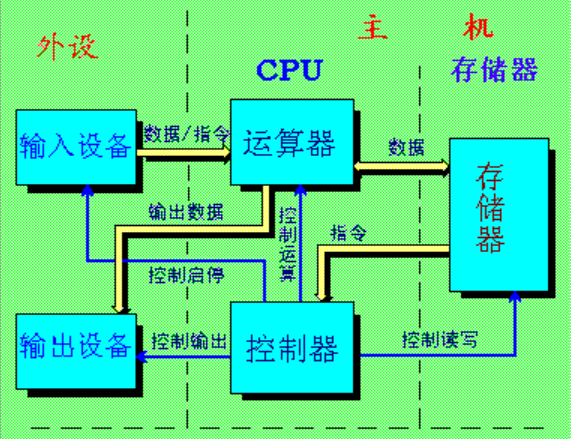
\includegraphics[scale=1]{part_8086CPU/part_8086CPU_pic/冯诺依曼计算机体系结构.png}
    \caption{冯诺依曼计算机体系结构图}
\end{figure}
\subsection{微机组成}
\begin{figure}[H]
    \centering
    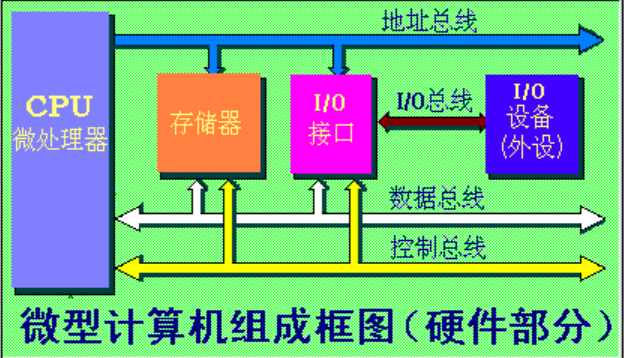
\includegraphics[scale=1]{part_8086CPU/part_8086CPU_pic/微机组成框图.png}
    \caption{微机组成框图}
\end{figure}
微型计算机由CPU微处理器、存储器、IO接口和IO设备(外设)组成
有4种总线
\begin{enumerate}
    \item 地址总线:连接CPU和存储器与IO接口
    \item 数据总线:连接CPU和存储器与IO接口
    \item 控制总线:连接CPU和存储器与IO接口
    \item IO总线:连接IO接口和IO设备
\end{enumerate}
工作过程
\begin{enumerate}
    \item 输入设备把指令送入IO接口,经过数据总线送入指定存储单元,存储器的地址由地址总线给出
    \item CPU从存储器取指令,产生地址、数据、控制信号,分别可以选中存储单元或端口、与选中的单元或接口交换数据、控制其他信号
\end{enumerate}
下面细讲各组成部分
\subsubsection{CPU}
即中央处理单元,计算机所有操作均在CPU的控制下进行,CPU型号直接决定了计算机的档次

Intel:
\begin{enumerate}
    \item 4004:4位微机
    \item 8085/8080:8位
    \item 8086/8088:16/准16位PC/XT机
    \item 80286:16位PC/XT机
    \item 80386/80486:32位机
    \item Pentium:奔腾32/64位机
\end{enumerate}
Motorola:6800(8位)——68000(16位)

Zilog:Z80(8位)——Z8000(16位)
\subsubsection{总线:BUS}
按传送的信息类型可以分为3类
\begin{enumerate}
    \item 数据总线:双向传送数据信息。可以连接多个设备,但是同一时间只能有一个设备在总线上(通过三态门控制)N根数据线可以同时传送N位信息。8086有16根,8088内部16,外部8根
    \item 地址总线:单向,用来寻址内存单元或IO端口。8086/8088都是20根
    \item 控制总线:输入输出,传送控制信号
\end{enumerate}
按规模、用途和应用场合可以分为3类
\begin{enumerate}
    \item 片级总线或元件级总线:用于芯片一级的互联,如CPU和存储器,CPU和IO接口
    \item 外部总线:也称为通信总线,用于微机和其他电子设备之间的连线
    \item 系统总线:也成为内总线和板级总线,用于微机中各插线板之间的连线
\end{enumerate}
\subsubsection{存储器:Memory}
用来存放数据和程序,每个存储单元存放一个字节,即8位bit。对每个存储单元编一个号,称为地址,地址单元和内容常常用16进制表示存储器中包含的字节数称为存储容量
\begin{figure}[H]
    \centering
    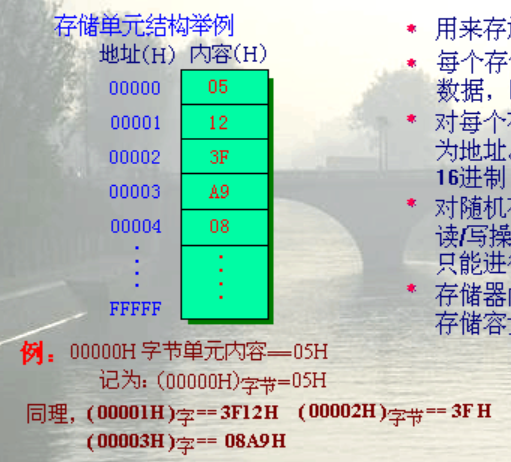
\includegraphics[scale=1]{part_8086CPU/part_8086CPU_pic/存储器结构举例.png}
    \caption{存储器结构举例}
\end{figure}
8086有20根地址线,可以直接寻址$2^{20}=1M$内存单元。使用了段加偏移的方法,一个物理地址有20位,可以表示为“段地址:偏移地址”=段地址*16+偏移地址

\noindentbfline{8086存储器}
一个程序可以有4个段,段名和段寄存器对应为
\begin{enumerate}\label{段寄存器4种}
    \item 代码段CS:code segment 将要执行的下一条指令一定是从CS:IP指示的单元中取出
    \item 数据段DS:data segment
    \item 堆栈段SS:stack segment
    \item 附加段ES:extra segment
\end{enumerate}
\subsubsection{IO接口}
为什么要有接口?因为外设与CPU交换数据的时候会带来一些问题
\begin{enumerate}
    \item 速度不匹配,一般是CPU远快于外设
    \item 信号电平不匹配
    \item 信号格式不匹配
    \item 时序不匹配
    \item 译码问题
\end{enumerate}
接口电路主要实现的功能
\begin{enumerate}
    \item 数据缓冲,使速度匹配:8255A通用并行接口、锁存器
    \item 电平转换:MC1488,MC1489,MAX233电平转换电路
    \item 串并行转换:8251A,8250串行接口芯片
    \item 数模模数转换:DAC0832,ADC0809
    \item 地址译码:74LS138
    \item 中断控制:8259A中断控制器
    \item 存储器直接数据传送控制:8237ADMA控制器
    \item 定时计数功能:8253,8254计数器/定时器
\end{enumerate}
\subsubsection{外设(即IO设备)}
输入设备:键盘、鼠标器、扫描仪、CD-ROM驱动器;

输出设备:CRT显示器、LPT打印机、扬声器、LED/LCD显示器
\subsection{微机系统组成}
\begin{equation}
    \begin{cases}
        \text{硬件}
        \begin{cases}
            \text{主机}
            \begin{cases}
                CPU\\
                \text{存储器}
            \end{cases}
            \text{各类接口芯片}\\
            \text{外设}
            \begin{cases}
                \text{输入设备}\\
                \text{输出设备}
            \end{cases}
        \end{cases}\\
        \text{软件}
        \begin{cases}
            \text{系统软件}
            \begin{cases}
                \text{操作系统:DOS、WINDOWS、UNIX}\\
                \text{汇编程序}\\
                \text{解释程序(对BASIC)}\\
                \text{编译程序(对高级语言)}
            \end{cases}\\
            \text{程序设计语言}
            \begin{cases}
                \text{机器语言}(\text{二进制码,计算机只认得这种语言})\\
                \text{汇编语言(符号语言)}\\
                \text{高级语言(C、FORTRAN、PASCAL)}
            \end{cases}\\
            \text{应用软件}
            \begin{cases}
                \text{软件包}\\
                \text{数据库}\\
                \text{文字处理软件、娱乐、教育等}
            \end{cases}
        \end{cases}
    \end{cases}
\end{equation}
\section{8086CPU系统}
\subsection{内部结构}
8086是16位,8088是准16位微处理器,都具有16位地址总线,可处理8或16位数据;外部都具有20根地址总线,可以直接寻址$2^{20}=1M$字节的内存空间,可以寻址$2^{16}=64K$个IO端口。

采用+5V供电,单相时钟

8086外部有16根地址总线,8088有8根,与外部传送数据时,都要执行外部总线周期。
\subsubsection{8086结构与原理}
\begin{figure}[H]
    \centering
    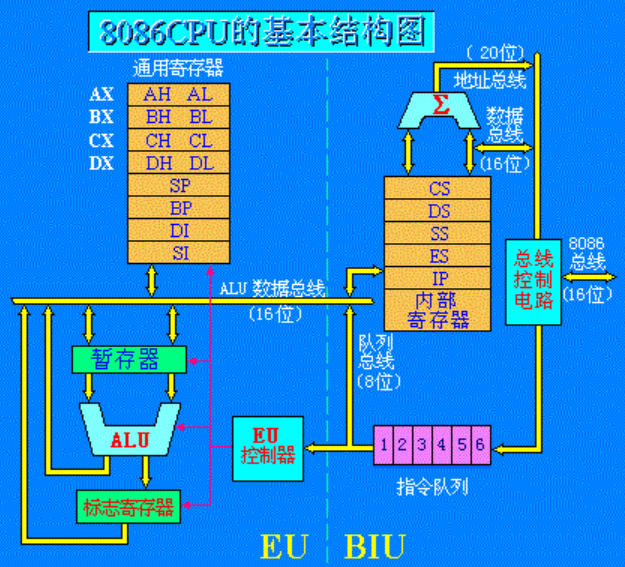
\includegraphics[scale=1]{part_8086CPU/part_8086CPU_pic/8086CPU基本结构.png}
    \caption{8086CPU基本结构}
\end{figure}
主要由两部分组成:

EU执行单元
\begin{enumerate}
    \item 负责执行全部指令
    \item 给BIU提供数据和地址信息
    \item 管理通用寄存器和标志寄存器,不直接和外部打交道
\end{enumerate}
BIU总线接口单元
\begin{enumerate}
    \item 执行所有的外部总线周期
    \item 负责与存储器,IO端口打交道
\end{enumerate}
工作流程
\begin{enumerate}
    \item 读操作:BIU根据CS:IP在地址加法器形成20位物理地址,通过总线控制电路从mem中取出指令,送到6字节的指令队列中等待执行
    \item EU从队列中取指令,译码后执行。此时没有用到总线,BIU可继续工作,把队列填满。如果EU没有向BIU申请读或写存储器或IO操作时,BIU空闲(*在执行指令时预先取下一条指令的技术称为流水线)
    \item 若遇到JMP或CALL指令,队列中的内容作废,从新的转移地址中取指令码
    \item ALU完成算数/逻辑运算后,将运算结果通过数据总线送到EU的通用寄存器或暂存器;或者送到BIU的内部寄存器再送到存储器或IO端口。本次操作的状态反映在标志寄存器FLAGS中
\end{enumerate}
\subsubsection{8088内部结构}
与8086基本一样,主要区别在于:
\begin{enumerate}
    \item 8088指令队列为4字节,而不是6字节
    \item 8088外部数据总线为8位而不是16位
\end{enumerate}
\subsubsection{总线周期简述}
总线周期:在8086中,BIU完成一次访问存储器或IO端口的时间称为总线周期。最基本的总线周期由$T_1$到$T_4$4个时钟周期组成,也称为$T_1$到$T_4$状态。
\begin{figure}[H]
    \centering
    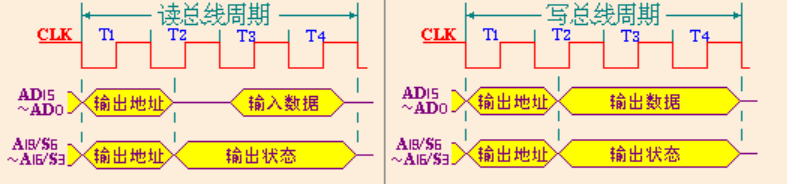
\includegraphics[scale=1]{part_8086CPU/part_8086CPU_pic/读周期和写周期.png}
    \caption{读周期和写周期}
\end{figure}
读周期:
\begin{enumerate}
    \item $T_1$状态通过4条地址/状态复用线和16条地址数据复用线(共20条线)向存储器输出指定地址
    \item $T_2$进入高阻态,缓冲一下,让AD地址数据复用线从输出地址变为输入数据信号。但是地址/状态复用线从$T_2$到$T_4$一直输出状态信号
    \item $T_3T_4$ 16条地址数据复用线接收指定单元内容
\end{enumerate}
\subsubsection{内部寄存器简述}
\begin{equation}
    \text{通用寄存器}
    \begin{cases}
        \text{数据寄存器}
        \begin{cases}
            \text{累加器AX}\\
            \text{基址寄存器BX}\\
            \text{计数寄存器CX}\\
            \text{数据寄存器DX}\\
        \end{cases}\\
        \text{指针和变址寄存器:涉及到存储器操作数时,可用的寄存器}
        \begin{cases}
            \text{堆栈指针SP:不能做通用寄存器}\\
            \text{基址指针BP}\\
            \text{源变址指针SI}\\
            \text{目的变址指针DI}
        \end{cases}
    \end{cases}\\
    \text{段寄存器}
    \begin{cases}
        \text{代码段指针CS}\\
        \text{数据段指针DS}\\
        \text{堆栈段指针SS}\\
        \text{附加段指针ES}
    \end{cases}\\
    \text{标志寄存器FLAGS}\\
    \text{指令指针IP}
\end{equation}
通用寄存器:16位寄存器用来存放数据和地址,8位的只能存放数据

数据寄存器隐含用途:
\begin{enumerate}
    \item AX:在字IO指令中,做16位数据寄存器;在字节乘法中存放乘积;在字节除法中存放被除数
    \item AH:字节除法中存放余数
    \item AL:字节IO指令中做8位数据寄存器;在字节乘法中存放乘数;在字节除法中存放商;BCD运算中必须将运算结果或被除数放在AL中才能用二-十进制调整指令调整;在XLAT指令中做指针和存放代码转换结果
    \item BX:做基地址指针;XLAT中存放表头地址
    \item CX:字符串操作和循环操作中做计数器
    \item CL:在算数逻辑移位和循环移位指令中做移位次数计数器
    \item DX:字乘法中存乘积的高半部分;字除法中存放被除数的高半部分和余数;在间接寻址的IO指令中做端口地址寄存器
\end{enumerate}
指针和变址寄存器隐含用途:
\begin{enumerate}
    \item SI:在字符串指令中做源串偏移地址指针
    \item DI:在字符串指令中做目的串偏移地址指针
    \item SP:在堆栈操作中指示栈顶位置
    \item BP:在堆栈操作中指示堆栈中一个数据区的偏移地址,可用于访问堆栈中的某个数据
\end{enumerate}
段寄存器:

计算机存储器中存放三类信息:代码信息,数据信息和堆栈信息,这三类信息存放在各自的内存区域中,用段寄存器来指示这些段的起始地址的高16位部分,一共有4种段寄存器\ref{段寄存器4种}

段寄存器和BX、BP、SI、DI等配合,可以构成多种寻址方式。例如CS:IP指出下一条要执行的指令的地址。SS:SP指向堆栈栈顶单元

标志寄存器:

16位FLAGS设置了9个标志位,其中6个为状态标志,用来反映上次运算结果的状态。另外三个为控制标志,用来控制CPU的某些操作
\begin{enumerate}
    \item OF(overflow)溢出标志:用于带符号数的运算,如果两个正数相加出现负数或者负数相加出现正数,则为1.(正确的结果也可能有进位,但是进位位自然丢失或给更高位)
    \item DF(direction)方向标志:控制SI、DI的变化方向。DF=0,则SI、DI自增;反之自减
    \item IF(interrupt)中断标志:STI指令使IF=1,允许CPU响应可屏蔽中断。CLI指令使IF=0,禁止CPU响应可屏蔽中断
    \item TF(trap)陷阱标志:TF=1,CPU处于单步工作方式,每执行一条指令自动内部中断,并打印信息,便于调试
    \item SF(sign)符号标志:数字的最高位MSB=1时,SF=1,表示结果为负值;MSB=0时,SF=0,表示结果为正值
    \item ZF(zero)零标志:运算结果为0时ZF=1
    \item AF(auxiliary)辅助进位标志:8位运算时,低半字节向高半字节有进位或借位时AF=1.16位运算时仅在低字节部分使用。一般用于BCD码运算的十进制调整(加6或减6)
    \item PF(parity)奇偶标志:算数逻辑运算时,结果有偶数个1时则PF=1,一般用来检验数据传输中的错误
    \item CF(carry)进位标志:最高位$D_7$或$D_{15}$产生进位或借位时CF=1
\end{enumerate}
指令指针

IP指针用来存放将要执行的下一条指令相对于现行代码段的偏移地址,用来控制指令序列的执行流程。

程序运行时,BIU自动对IP进行修改,使它始终指向下一条指令的地址。程序不能直接访问IP,只能由CPU自动控制
\subsection{存储器基础}
存储器主要用来存放程序和数据,存储容量和存取速度是决定性指标。内存容量一般指RAM大小
\subsubsection{存储器分类}
\begin{equation}
    \begin{cases}
        \text{内存}
        \begin{cases}
            RAM
            \begin{cases}
                SRAM\\
                DRAM
            \end{cases}\\
            ROM
            \begin{cases}
                ROM\\
                PROM\\
                EPROM\\
                E2PROM
            \end{cases}
        \end{cases}\\
        \text{外存}
        \begin{cases}
            \text{硬盘}\\
            \text{软盘}\\
            \text{磁带}\\
            \text{光盘}
        \end{cases}\\
        \text{高速缓冲存储器Cache}
    \end{cases}
\end{equation}
\subsubsection{8086分段概念}
为什么要分段?因为地址线有20根,但是CPU寄存器只有16位。

怎么分段?一个现行程序可以分为DS、CS、SS和ES四段,凡是能被16(或10H)整除的地址处均可分段。如00000H,00010H,00150H等

各段之间可以相互独立也可以相互覆盖

分段的好处?
\begin{enumerate}
    \item 大部分指令不涉及段寄存器的值,仅改变偏移量,这样可以缩短指令长度,提高运算速度
    \item 内存分段为程序的浮动装配创造条件
\end{enumerate}
\subsubsection{8086存储器结构}
8086可直接寻址的1MB内存分成2个512K的存储体,$A_0=0$选到偶地址体,$A_0=1$选到奇地址体。

CPU访问存储器都是从偶地址体开始的,以字为单位进行操作。读00000字时,从00000开始读两个字节,读出来的是(00001)(00000)代表的字;读00003字时,从00004开始读到00003,即读出内容为(00004)(00003)代表的字。

\noindentbfline{8086系统与存储器的连接}
\begin{enumerate}
    \item 每个存储器单元有8根数据线,奇地址体与CPU的高8位相连,偶地址体与低8位相连
    \item 用$A_0$和$\overline{BHE}$(Bus High Enable)来控制地址体的选中与否
\end{enumerate}
\begin{table}
    \centering
    \begin{tabular}[h]{c|c|c}
        \hline
        $\overline{BHE}$ & $A_0$ & 操作 \\ \hline
        0 & 0 &奇偶地址体都被选中,读字\\\hline
        0 & 1 &读偶地址体字节\\\hline
        1 & 0 &读奇地址体字节\\\hline
        1 & 1 &无操作 \\ \hline
    \end{tabular}
\end{table}
\subsubsection{8086堆栈操作}
一个堆栈不超过一个段的指示范围($2^{16}=64K$),由SS给出段基地址,SP存放偏移地址,指示栈顶位置,$SP\leq FFFEH$

堆栈的基本处理单元是字,压栈时,一个字的高8位先入栈,低8位后入栈,SP的值减二(注意16进制减法的不同)
\subsection{引脚功能}
\subsubsection{8086CPU引脚}
\noindentbf{$AD_{15}-AD_{0}$地址/数据总线}
分时复用:在总线周期的$T_1$状态,传送存储器或IO端口的地址信息,然后在ALE信号控制下用锁存器将$A_{15}-A_{0}$锁存住

$T_2$状态:读总线周期下为高阻态,写总线周期下,传送数据信号$D_{15}-D_0$

$T_3-T_4$状态:传送传送数据信号$D_{15}-D_0$

\noindentbf{INTR中断请求}
为高电平时,表示外部向CPU发送中断请求信号。CPU在每条指令的最后一个时钟周期都要对其信号进行采样,若为1,CPU的IF=1,则CPU转入中断响应周期

\noindentbf{NMI不可屏蔽中断}
CPU一旦检测到NMI的上跳变信号,则执行完当前指令后,进入类型2的不可屏蔽中断。这类中断不受IF影响,不能用软件屏蔽。

\noindentbf{CLK}
由外部时钟信号8284提供,基本在MHz级别

\noindentbf{$A_{19}S_{6}-A_{16}S_{3}$地址/状态总线}
分时复用:在总线周期的$T_1$状态做地址线用,可用于访问存储器,但是访问IO端口只用到低16位地址线,所以这四根线无效

$T_2-T_4$状态:输出状态信息
\begin{enumerate}
    \item $S_6=0$
    \item $S_5=1$允许可屏蔽的中断请求,$S_5=0$禁止可屏蔽的中断请求
    \item $S_4S_3$段寄存器状态线,从00到11分别表示当前正在使用的段寄存器为ES,SS,CS,DS
\end{enumerate}
\noindentbf{$\overline{BHE}/S_7$总线高位有效/状态线}
分时复用:$T_1$输出有效的$\overline{BHE}$信号。其他时候输出$S_7$,在8086中$S_7$无意义

\noindentbf{$MN/\overline{MX}$最小/最大模式} 

\noindentbf{$\overline{RD}$读信号}
执行读指令时该引脚变为低电平,到底是读存储器还是读IO取决于$M/\overline{IO}$信号

\noindentbf{READY准备好信号}由8284时钟信号产生器产生,一般CPU与低速外设交换数据时要等外设,此时READY变低电平,这样可以在$T_3$后插入若干等待周期$T_w$;READY变为高电平后,下一个周期进入$T_4$

\noindentbf{$\overline{TEST}$测试信号}CPU执行WAIT指令时,每隔5个T就检测一次该引脚,若为高电平(无效)则进入空闲周期,反之继续执行下一条指令

\noindentbf{RESET复位信号}高电平有效,至少维持4个时钟周期。复位时:
\begin{enumerate}
    \item CPU立即中止所有操作,总线无效
    \item IP,DS,ES,SS,FLAGS清零,CS=FFFFH,复位结束后,CS:IP=FFFF:0000H,CPU从这里开始执行程序,所以可在这里安排一条JMP RESET
    \item 指令队列清空
\end{enumerate}
\subsubsection{8088CPU引脚}
\noindentbf{$A_{15}-A_{8}$地址线}不与数据线复用,因为8088只需要8根数据线

\noindentbf{$SS_0$(High)}最小模式下为状态信号,与$IO/\overline{M}$,$DT/\overline{R}$一起决定现行总线周期的状态。最大模式下接高电平。

\noindentbf{$IO/\overline{M} (S_2)$}在8088中为1时访问IO,为0时访问存储器。在8086中反之
\subsection{工作模式}
$MN/\overline{MX}$接高电平时工作于最小模式:
\begin{enumerate}
    \item 系统中只有一个8086或8088微处理器
    \item 所有总线控制信号均由CPU直接产生或接收
\end{enumerate}
$MN/\overline{MX}$接低电平时工作于最大模式:
\begin{enumerate}
    \item 系统中允许多个处理器共同工作
    \item 有的控制信号由CPU直接产生,有的由8288总线控制器译码后产生
    \item 单个CPU也可以工作在最大模式
\end{enumerate}
两者的共同点:
\begin{enumerate}
    \item 都需要用地址锁存器8282/8283或74LS373(因为20位地址线,所以都要用三片芯片),使地址数据线先传送地址并锁存,再传送数据信号
    \item 都需要使用8286/8287或74LS245(8086用两片,8088用一片)控制数据传送的方向,同时增强数据总线的驱动力,在小系统中可以不用数据收发器。
\end{enumerate}
\subsubsection{8086最大模式}
\begin{figure}[H]
    \centering
    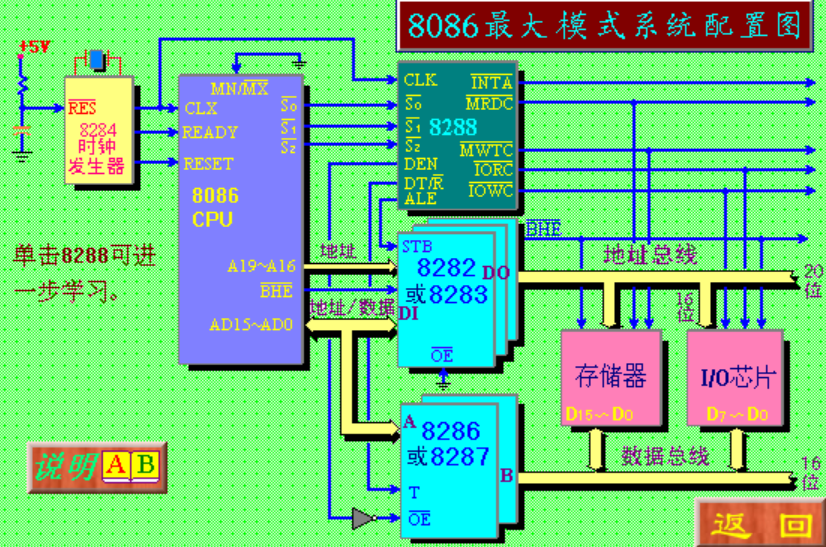
\includegraphics[scale=1]{part_8086CPU/part_8086CPU_pic/8086最大模式系统配置图.png}
    \caption{8086最大模式系统配置图}
\end{figure}
特征:
\begin{enumerate}
    \item $MN/\overline{MX}$接地
    \item 增加总线控制器8288来产生原来由CPU产生的控制信号
    \item 8288产生的ALE(地址锁存允许)、DEN(数据传送允许)和$DT/\overline{R}$(数据收发允许)三种信号与CPU一致
\end{enumerate}
\noindentbf{8288总线控制器}
接收时钟产生器送出的CLK信号,其频率与CPU的CLK相同。同时还接收CPU送来的状态信号,从输出端输出各种控制信号
\begin{enumerate}
    \item $DT/\overline{R}$,$ALE$:与最小模式信号相同
    \item DEN:与最小模式的$\overline{DEN}$相位相反
    \item $\overline{MRDC}$:存储器读,相当于$\overline{RD},M/\overline{IO}$结合,选中存储器。引到系统总线上命名为$\overline{MEMR}$
    \item $\overline{MWTC}$:存储器写,相当于$\overline{WR},M/\overline{IO}$结合,选中存储器。引到系统总线上命名为$\overline{MEMW}$
    \item $\overline{IORC}$:IO读,相当于$\overline{RD},M/\overline{IO}$结合,选中IO端口。引到系统总线上命名为$\overline{IOR}$
    \item $\overline{IOWC}$:IO写,相当于$\overline{WR},M/\overline{IO}$结合,选中IO端口。引到系统总线上命名为$\overline{IOW}$
    \item $\overline{INTA}$:中断响应信号
    \item *$\overline{AIOWC}$:超前写IO命令,与$\overline{IOWC}$相比,8288提前一个时钟周期向IO端口发出写命令。可以使较慢的设备提前一个周期进入写操作。用于PC机中。
    \item *$\overline{AMWC}$:超前写存储器命令,与$\overline{MWTC}$相比,8288提前一个时钟周期向存储器发出写命令
\end{enumerate}
\subsubsection{8086最小模式}
\begin{figure}[H]
    \centering
    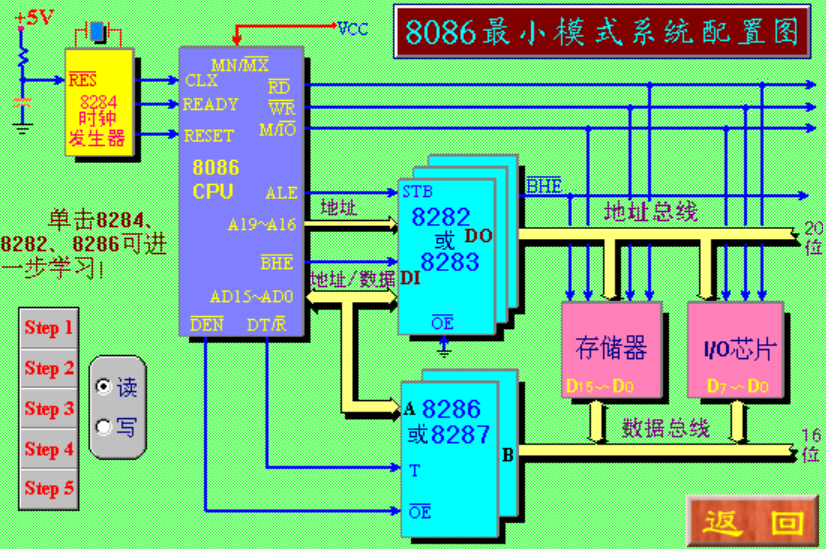
\includegraphics[scale=1]{part_8086CPU/part_8086CPU_pic/8086最小模式系统配置图.png}
    \caption{8086最小模式系统配置图}
\end{figure}
读存储器操作流程(读IO仅在第一步$M/\overline{IO}=0$处不一样)
\begin{enumerate}
    \item $M/\overline{IO}$置1选中存储器,$DT/\overline{R}$置零,使8286T引脚为零,使CPU准备接收数据
    \item 地址信号和$\overline{BHE}$输出给8282,同时送出一个ALE正脉冲,在ALE下降沿锁存
    \item 三态门打开,8282输出地址信号和$\overline{BHE}$到存储器某一指定单元
    \item CPU发出$\overline{RD}=0$读信号,同时CPU的$\overline{DEN}=0$使8286可以接收数据,且8286的T=0,允许接收数据
    \item 从选中的存储器单元中读出来送给8286,再送给CPU的$AD_{15}-AD_{0}$
\end{enumerate}

写存储器操作流程(写IO仅在第一步$M/\overline{IO}=0$处不一样)
\begin{enumerate}
    \item $M/\overline{IO}$置1选中存储器,$DT/\overline{R}$置1,使8286T引脚为1,使CPU准备发送数据
    \item 地址信号和$\overline{BHE}$输出给8282,同时送出一个ALE正脉冲,在ALE下降沿将20位地址和$\overline{BHE}$锁存
    \item 8282三态门打开,8282输出地址信号和$\overline{BHE}$到存储器某一指定单元
    \item CPU发出$\overline{WR}=0$读信号,同时CPU的$\overline{DEN}=0$使8286可以接收数据,且8286的T=1,允许发送数据
    \item CPU通过$AD_{15}-AD_{0}$把要写入的数据送给8286,再送到存储单元
\end{enumerate}
\noindentbf{8282地址锁存器(或用74LS373)}
\begin{figure}[H]
    \centering
    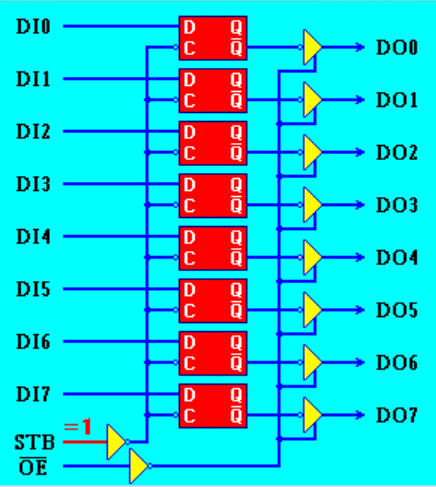
\includegraphics[scale=1]{part_8086CPU/part_8086CPU_pic/8282地址锁存器.png}
    \caption{8282地址锁存器}
\end{figure}
由8个D触发器和8个三态门组成,有STB和$\overline{OE}$两个控制端。STB=1时D触发器透明,STB产生下降沿时,锁存,STB=0时D端变化Q不变;当$\overline{OE}=0$时三态门开启,可以把$\overline{Q}$反相后输出,相当于输出Q,当$\overline{OE}=1$时不能输出

\noindentbf{8286数据收发器(或用74LS245)}
\begin{figure}[H]
    \centering
    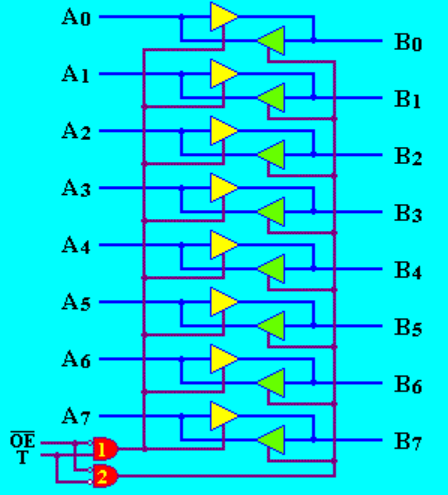
\includegraphics[scale=1]{part_8086CPU/part_8086CPU_pic/8286数据收发器.png}
    \caption{8286数据收发器}
\end{figure}
由8组首尾相连的反相器组成。$\overline{OE}=1$时禁止收发数据,输出低电平;$\overline{OE}=0$时允许收发数据,若T=1,传送方向为A到B(发送),反之为接收。

\noindentbf{8284时钟产生器}
\begin{figure}[H]
    \centering
    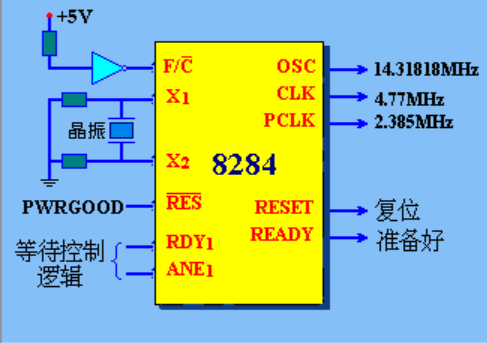
\includegraphics[scale=1]{part_8086CPU/part_8086CPU_pic/8284时钟发生器.png}
    \caption{8284时钟发生器}
\end{figure}
\begin{enumerate}
    \item $F/\overline{C}=0$时,输入频率由晶振决定,可以输出三种脉冲信号
    \item $\overline{RES}$接PWRGOOD,系统加电,四种直流输出电压($\pm 5,\pm 12$)正常后,送出PWRGOOD,经8284同步,产生RESET送到CPU的RESET引脚引起复位
    \item RDY、AEN与外部等待逻辑电路相连,经8284同步后可以产生READY信号送给CPU,以产生等待周期$T_w$
\end{enumerate}
\subsubsection{8088最大模式}
地址是20位,但无$\overline{BHE}$信号,数据线只有8位,所以8286只用一片。地址/数据复用线为$AD_7-AD_0$
\subsubsection{8088最小模式}
也要3片8282,在小系统中可以不用8286
\subsection{典型时序}
\subsubsection{读总线周期}
总线周期分为4个时钟周期,都是在时钟的下降沿触发。
\begin{figure}[H]
    \centering
    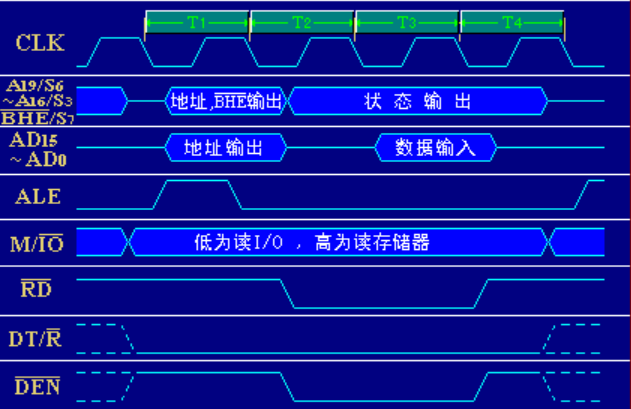
\includegraphics[scale=1]{part_8086CPU/part_8086CPU_pic/读总线周期.png}
    \caption{读总线周期}
\end{figure}
\subsubsection{写总线周期}
\begin{figure}[H]
    \centering
    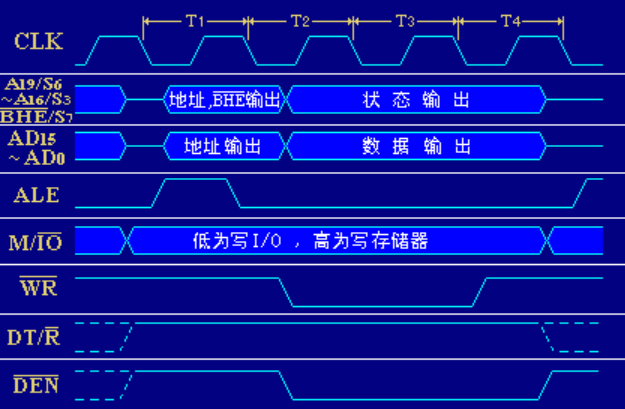
\includegraphics[scale=1]{part_8086CPU/part_8086CPU_pic/写总线周期.png}
    \caption{写总线周期}
\end{figure}
\subsection{存储器设计}
\subsection{SRAM 6264}
容量大小:8K×8

引脚及功能:
\begin{enumerate}
    \item $A_{12}-A_0$:13根地址线,选择芯片中$2^{13}$个存储单元中的任一个单元
    \item $I/O_7-I/O_0$:八根双向数据线,并行送数据
    \item $\overline{WE}$:写入允许信号
    \item $\overline{OE}$:读出允许信号
    \item $\overline{CE_1},\overline{CE_2}$:片选信号,两者均为低电平才能对芯片进行读写操作。其中一个作奇偶选择信号用。
\end{enumerate}
\subsection{SRAM 2114}
容量大小:1K×4

引脚及功能:
\begin{enumerate}
    \item $A_{9}-A_0$:13根地址线,选择芯片中$2^{13}$个存储单元中的任一个单元
    \item $I/O_4-I/O_0$:八根双向数据线,并行送数据
    \item $\overline{WE}$:写入允许信号
    \item $\overline{CS}$:片选信号
\end{enumerate}
\subsection{EPROM 2764}
EPROM允许用户将写入的内容用专门的擦除器擦除,允许反复擦除与重写。但是2764在正常使用时只能读出。
容量大小:8K×8

引脚及功能:
\begin{enumerate}
    \item $A_{12}-A_0$:13根地址线,选择芯片中$2^{13}$个存储单元中的任一个单元
    \item $O_7-O_0$:八根双向数据线,并行送数据
    \item $\overline{OE}$:读出允许信号
    \item $\overline{CE}$:片选信号
    \item PGM:编程脉冲控制
    \item $V_{pp}$:编程电压输入
    \item $V_{cc}$:工作电压,接+5V
\end{enumerate}
*编程方式时的引脚状态
\begin{enumerate}
    \item $A_{12}-A_0$:选中存储单元,逐字编程
    \item $\overline{OE}$:接+5V
    \item $\overline{CE}$:接+5V
    \item PGM:对每个单元编程时,从该引脚上输出一个50ms宽的正脉冲
    \item $V_{pp}$:接+21V到+25V
    \item $V_{cc}$:工作电压,接+5V
\end{enumerate}
\subsection{存储器系统连线图}
\begin{figure}[H]
    \centering
    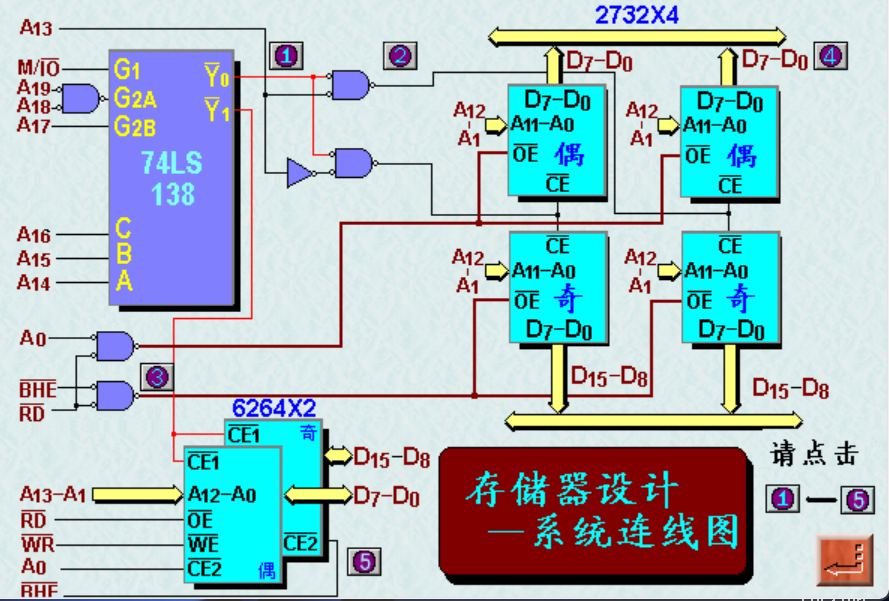
\includegraphics[scale=1]{part_8086CPU/part_8086CPU_pic/存储器系统连线图.png}
    \caption{存储器系统连线图}
\end{figure}
